\documentclass[a4paper,twoside,final]{article}
%----Eingebundene Bibliotheken-----
\usepackage[ngerman]{babel}         % Deutsches Sprachpaket
\usepackage[utf8]{inputenc}         % Eingaben codieren
\usepackage[T1]{fontenc}            % Umlaute codieren, Silbentrennung
\usepackage{amsmath, amssymb}       % Mathe
\usepackage{amsthm,amstext,amsxtra} % Symbole für Mathe
\usepackage{mathtools}              % \Aboxed Boxen in align
\usepackage{wrapfig}                % Bilder umfließen
\usepackage{svg}                    % Vektorgraphiken einbinden
\usepackage{geometry}               % Papierformat
\usepackage{tabularx}               % Tabellen
\usepackage{xcolor,colortbl}        % Farben
\usepackage{graphicx}               % Für Limes Definition wichtig
\usepackage{soul}                   % Unterstreichungen
\usepackage[section]{placeins}      % \Floatbarrier
\usepackage{wrapfig}                % Bilder umfließen
\usepackage{enumerate}              % Aufzählungen
\usepackage{footnote}               % Fußzeilen
\usepackage{booktabs}               % publication quality tables
\usepackage[hyphens]{url}           % \url{}
\usepackage{bm}                     % bold symbols \bm{r}
\usepackage{dsfont}                 % identity matrix \mathds{1}
\usepackage{enumitem}               % itemize Umgebungen customizen
\usepackage{esint}                  % Doppelintegrale
\usepackage{fancyhdr}               % schöne Kopf- und Fußzeilen
\usepackage{lmodern}
\usepackage{tikz}
\usepackage{pgfmath, pgfplots}
\usepackage[labelfont=bf]{subcaption}
\usepackage[square,numbers,sort&compress]{natbib}
\usepackage{mhchem}                 % Chemistry Package
\usepackage{physics}
\usepackage{chemfig}
\usepackage[detect-all,
            locale=DE,binary-units,
            exponent-product=\cdot
            ]{siunitx}              % \SI{12}{\gram}
%siunitx stellt für Tabellen den Spaltentyp S bereit ==> Ausrichtung an Dezimaltrennzeichen
\usepackage[position=below,
            tableposition=top,
            format=hang,
            labelfont=it,
            labelfont=bf,
            ]{caption}              % Settings für Captions
\captionsetup[wrapfigure]{name=Abb.}
\usepackage[europeanvoltages,
            europeancurrents,
            europeanresistors,
            americaninductors,
            europeanports
            ]{circuitikz}           % Schaltungen
\usepackage{chngcntr}               % vor hyperref laden!
  \counterwithin*{equation}{section}
  \counterwithin*{figure}{section}
  \counterwithin*{table}{section}

\usepackage[final,
            pdfauthor={Martin Beyer, Vanessa Huth},
            pdfsubject={Fortgeschrittenen-Praktikum},
            pdffitwindow=true,      % resize document window
            pdftitle={Fortgeschrittenen-Praktikum},
            bookmarks=true,         % lesezeichen-Liste
            bookmarksopen=true,     % Lesezeichen geöffnet
            bookmarksopenlevel=1,
            bookmarksnumbered=true,
            colorlinks=true,        % fuer Druckversion auf "false"
            linkcolor=blue,         % Table of Contents, Footnotes
            urlcolor=blue,          % fuer eingebunden URLs
            citecolor=blue,         % Equations, References
            filecolor=blue,
            pdfborder={0 0 0},      % keine Rahmen um Links: {0 0 0}
            ]{hyperref}


% Commands
\renewcommand{\sfdefault}{lmss}     % latin modern sans serif
\newcommand{\R}{\mathbb{R}}         % Reelle Zahlen
\newcommand{\N}{\mathbb{N}}         % Natürliche Zahlen
\newcommand{\C}{\mathbb{C}}         % Komplexe Zahlen
\newcommand{\de}{\mathrm{d}}      % Differential
\newcommand{\entspricht}{\mathrel{\widehat{=}}}

\DeclareSIUnit{\eV}{\text{eV}}
\DeclareSIUnit{\voltpeakpeak}{\volt{\textsubscript{pp}}}

% Dokumenteneinstellungen
\setlength{\parindent}{0px}         % remove indent in new paragraph
\setlength{\parindent}{0px}         % keine Absätze durch Leerzeilen im Code
\emergencystretch=1em % Definiert den Leerraum, der innerhalb einer Zeile zusätzlich verteilt werden darf.
\setlength{\topmargin}{-5mm} % 210mm = 8.2677165in
\newlength{\mylength}
\setlength{\mylength}{\paperwidth}
\addtolength{\mylength}{-2in} % standardmäßig wird den Seitenrändern jeweils noch 1in = 25.4mm hinzuaddiert
\setlength{\textwidth}{145mm}
\setlength{\textheight}{230mm}
\addtolength{\mylength}{-\textwidth}
\setlength{\oddsidemargin}{10mm}
\addtolength{\mylength}{-\oddsidemargin}
\setlength{\evensidemargin}{\mylength}
\setlength{\marginparwidth}{1.7cm}
\interfootnotelinepenalty=10000

% Umdefinition von \textcolor ********************************************************
\makeatletter
\renewcommand*{\@textcolor}[3]{%
	\protect\leavevmode
	\begingroup
	\color#1{#2}#3%
	\endgroup
}
\makeatother
% Damit das auch im Mathemodus anwendbar ist und dort z.B. die Leerzeichen nicht wie im Textmodus gesetzt werden.

\pgfplotsset
{compat=newest, % aktuelle Version: 1.16 [29.05.2018]
	/pgf/number format/.cd, % cd steht fuer current directory
	%  	use comma, % Komma als Dezimaltrennzeichen %%% UNCOMMENT THIS !!!
	1000 sep={} % Legt das Tausendertrennzeichen fest
}
%\usepgfplotslibrary{external} % Section 7.1.1 Using the Automatic Externalization Framework of TikZ
%\tikzexternalize[prefix=FiguresTikZ/] % activate externalization! Use subdirectory [FiguresTikZ]
\usepgfplotslibrary{fillbetween}
\usepgfplotslibrary{polar}
\usetikzlibrary{arrows.meta}
\usetikzlibrary{calc}
\usetikzlibrary{datavisualization.formats.functions}
\usetikzlibrary{intersections}
\usetikzlibrary{patterns}
\usetikzlibrary{pgfplots.colormaps}
\usetikzlibrary{plotmarks}
\usetikzlibrary{shapes.geometric}

% Generelle Festlegung des Styles fuer Blockschemata (Plaene fuer Regelkreise, etc.)
\tikzstyle{block} = [draw, fill=blue!20, rectangle, minimum height=1cm, minimum width=1cm]%, minimum width=6em]
\tikzstyle{sum} = [draw, fill=blue!20, circle, node distance=1cm]
\tikzstyle{input} = [coordinate]
\tikzstyle{output} = [coordinate]
\tikzstyle{pinstyle} = [pin edge={to-,thin,black}]

\begin{document}
\setlength{\marginparsep}{2em}
\renewcommand{\theequation}{\arabic{section}.\arabic{equation}}
\renewcommand{\thefigure}{\arabic{section}.\arabic{figure}}
\renewcommand{\thetable}{\arabic{section}.\arabic{table}}

% Anfang ********************************************************
\begin{center}
\thispagestyle{empty}
  
\includegraphics[width=0.75\textwidth]{../UniJena_BildWortMarke_black.pdf}\\[4em]
  \Large
  Ausarbeitung zum Versuch\\[2em]
  \Huge
  Radiowellen auf Leitungen\\
  und im freien Raum\\
  \vspace{2cm}
  \Large
  Martin Beyer und Vanessa Huth\\[2em]
  Abgabe: 03. Dezember 2019\\[2em]
  Betreuer: \\[5em]
  \begin{flushleft}
  	Bewertung und Ausarbeitung:\\[2em]
		Protokollführung und Form:\\[1em]
		Ergebnisse, Auswertung und Interpretation:\\[1em]
		Bemerkungen und Hinweise des Betreuers:
  \end{flushleft}
\end{center}
\clearpage

\pagestyle{fancy}
\renewcommand{\headrulewidth}{0pt}
\renewcommand{\footrulewidth}{0.5pt}
\renewcommand{\sectionmark}[1]{\markright{#1}}
\fancyhead[RO,LE]{\textbf{Radiowellen}}
\fancyhead[RE,LO]{\rightmark}
\fancyfoot[LE,RO]{\bfseries\thepage}
\fancyfoot[CO,CE]{Protokoll}
\renewcommand{\headrulewidth}{0.5pt}
\renewcommand{\footrulewidth}{0.5pt}

\setcounter{equation}{0}
\setcounter{figure}{0}

% *********************************************
% ***** KAPITEL 1 *****************************
% *********************************************
\tableofcontents
\newpage
\section{Aufgabenstellung} \label{sec:Aufgabenstellung}
\subsection{Elektromagnetische Wellen auf Leitungen}
\paragraph{Sinussignale}$~$\\
Es wird Das Verhalten von Sinussignalen auf der Leitung bei verschiedenen Kabelsorten und -anordnungen im Bereich von $1\hdots\SI{100}{\mega\hertz}$ untersucht. Es folgt eine grafische Darstellung mit Bestimmung des Verkürzungsfaktors, der Ausbreitungsgeschwindigkeit und Permittivität für die verwendeten Kabel.
\paragraph{Rechtecksignale}$~$\\
Es werden Rechtecksignale erzeugt und am \textit{Scope} mit verschiedenen Eingangswiderständen oszillographiert. Dabei werden Koaxial-Kabel unterschiedlicher Länge verwendet. Es erfolgt ebenfalls die Bestimmung der Ausbreitungsgeschwindigkeit, des Verkürzungsfaktors und der Permittivität der Anordnungen.
\paragraph{Messungen am Koaxialkabel}$~$\\
Es wird experimentell der Wellenwiderstand eines RG58 Koaxialkabels mit Rechteckimpulsen unter Verwendung verschiedener Methoden bestimmt. Zudem wird die Dispersion und das verwendete Dielektrikum des Koaxialkabels bestimmt. Für ein unbekanntest Kabelstück soll ebenfalls das Dielektrikum bestimmt werden. In einem LAN-Netzwerkkabel wird der Wellenwiderstand und der Frequenzgang bestimmt und mit dem Koaxialkabel verglichen.

\subsection{Modulation}
\paragraph{Amplitudenmodulation}$~$\\
Additive und multiplikative Amplitudenmodulation wird mithilfe von LabView simuliert. Parallel dazu wird die Modulation im Experiment realisiert und der Modulationsgrad varriert. Das amplitudenmodulierte Signal wird mithilfe eines Hüllkurvendemodulators demoduliert.
\paragraph{Frequenzmodulation}$~$\\
Die Frequenzmodulation wird mit LabView simuliert und parallel im Experiment realisert.

\subsection{Radiowellen im freien Raum}
Es sollen die Grundlagen der Dimensionierung und Berechnung von einer Halbwellendipolantenne und Viertelwellenstrahler recherchiert werden.\\
Mithilfe eines Reflektometers wird der Reflexionsfaktor eines Koaxialkabels in Abhängigkeit von der Frequenz $\SI{10}{\mega\hertz}\hdots\SI{1}{\giga\hertz}$ bestimmt. Es soll untersucht werden, welche Möglichkeiten zur messung der Ausbreitungsgeschwindigkeit in Luft realisiertbarsind.\\
Weiterhin wird ein amplitudenmoduliertes Signal über einen Halbwellendipol abgestrahlt, empfangen und demoduliert. \\
Zudem wird eine Übersicht der verwendeten Funkfrequenzen und deren Verwendungszweck erstellt. Das örtliche Frequenzspektrum und die zugehörigen Funkdienste werden bestimmt.\\
Die Ausbreitung von EM-Wellen in Wasser wird unterrsucht.
%% More to do
%%
%%


% *********************************************
% ***** KAPITEL 2 *****************************
% *********************************************
\newpage
\section{Grundlagen} \label{sec:Grundlagen}

\subsection{Elektromagnetische Wellen auf Leitungen}
Die Leitungstheorie befasst sich mit Vorgängen auf Leitungen deren Länge sich in der Größenordnung der Wellenlänge
des zu übertragenden Signals befindet, wodurch sie unter anderem in der Hochfrequenztechnik anzuwenden ist. Beispielsweise hat eine elektromagnetische Welle der Frequenz $\nu = \SI{100}{\mega\hertz}$ eine Wellenlänge von $\SI{3}{\metre}$.\\
Es gilt das Leistungsanpassungsgesetz mit $Z_Q$ als Quellwiderstand und $Z_A$, dem Abschlusswiderstand. Bei $Z_Q = Z_A$ entsteht eine Leistungsanpassung, d.\,h. maximale Leistung wird übertragen.\\
Im Hochfrequenzbereich muss eine weitere Größe, der \textit{Wellenwiderstand} $Z_L$ der Leitung berücksichtigt werden. Hierbei wird gefordert, dass $Z_L = Z_A$ idealerweise gelten muss, um stehende Wellen zu vermeiden. 
\begin{figure}[htp]
    \centering
    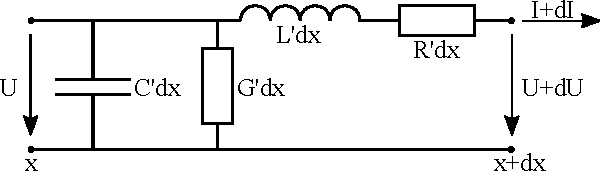
\includegraphics[width=0.8\textwidth]{Schaltungen/Ersatzschaltbild.pdf}
    \caption{Ersatzschaltbild eines homogenen Leitungsstücks von $x$ bist $x+\de x$.}
    \label{fig:Ersatzschaltbild}
\end{figure}\\


\subsection{Modulation}
Als Modulation wird das Aufprägen einer Information auf eine Trägerschwingung bezeichnet. Dabei wird das zu übertragene Nutzsignal in einen definierten höheren Frequenzbereich verschoben. Dies wird benötigt, weil der direkte Übertragungsweg des Signals durch ein Medium wie z.\,B. Schall häufig nicht über lange Strecken möglich ist. Im Allgemeinen erfolgt die Signalübertragung über einen Kanal wie Luft oder Kabel. Im Kanal tritt eine frequenzabhängige Dämpfung auf, weshalb das Signal auf eine Frequenz innerhalb eines dämpfungsarmen Frequenzfensters moduliert wird. Für das Nutzsignal und den Träger lassen sich folgende Formeln aufstellen.
\begin{align}
    U_\text{Nutz}(t) &= U_\text{N}\cdot\cos(\omega_\text{N}t) & \text{Spannung Nutzfrequenz}\\
    U_\text{Träger}(t) &= U_\text{T}\cdot\cos(\omega_\text{T}t) & \text{Spannung Trägerfrequenz}
\end{align}
Der Träger wird benötigt, um die Information des Nutzsignals durch spätere Demodulation wieder zu erhalten.\\
Die Mischung zweier Signale wird technisch auf gleiche Weise realisiert wie die Modulation. Bei der Mischung wird nur eine der entstehenden Frequenzen weiter benutzt, während bei der Modulation mehrere Mischprodukte weiter verwendet werden.
\subsubsection{Amplitudenmodulation}
Bei der Amplitudenmodulation wird das Signal in der Amplitude der Trägerschwingung kodiert. Die Amplitude des modulierten Signals ändert sich mit der Frequenz des Nutzsignals, während die Schwingungsfrequenz durch den Träger vorgegeben wird. Es lassen sich zwei verschiedene Verfahren unterscheiden.
\paragraph{Additive Amplitudenmodulation}
Hierbei handelt es sich um die am einfachsten realisierbare Variante. Die zu modulierenden Signale werden überlagert und anschließend an einer Kennlinie (Diode oder Transistor) mit exponentiellen Verlauf verzerrt. Dabei entstehen neue Frequenzkomponenten.
\begin{align}
  U_\text{AM}(t) = U_\text{T}\cos(\omega_\text{T}t) + U_\text{N}\cos(\omega_\text{N}t)\cdot U_\text{T}\cos(\omega_\text{T}t)
\end{align}
Neben der Trägerfrequenz $\omega_\text{T}$ entstehen im amplitudenmodulierten Signal zwei weitere Frequenzen. Diese Schwebungsfrequenzen $\omega_\text{T} \pm \omega_\text{N}$ werden als Seitenbänder bezeichnet.
\begin{align}
  U_\text{oberes Seitenband}\cos(\omega_\text{T} + \omega_\text{N})\\
  U_\text{unteres Seitenband}\cos(\omega_\text{T} - \omega_\text{N})
\end{align}
Üblicherweise wird die Trägerfrequenz $\omega_\text{T}$ so gewählt, dass sie viel größer als die Signalfrequenz ist, $\omega_\text{S} \ll \omega_\text{T}$, weshalb alle auftretenden Frequenzen im Größenbereich der Trägerfrequenz liegen.\\
Eine weitere charakteristische Größe stellt der Modulationsgrad $M$ dar. Dieser ist definiert als Verhältnis der Hüllkurvenamplitude zur Trägeramplitude und berechnet sich folgendermaßen
\begin{align}
  M = \frac{U_N}{U_T} = \frac{\text{max}-\text{min}}{\text{max}+\text{min}},
\end{align}
wobei die beiden Größen in Abbildung~\ref{fig:Amplitudenmodulation} eingezeichnet sind.
\begin{figure}[htp]
    \centering
        \begin{center}
	\newcommand\maxt{2} % in [s]
	\newcommand\fTraeger{20} % in [Hz]
	\newcommand\fSignal{1.5} % in [Hz]
	\newcommand\Modulationstiefe{50} % in Prozent

	\begin{tikzpicture}[trim axis left, trim axis right]
  	\begin{axis}[
    	clip=false,
    	width=0.9\textwidth, height=0.3\textwidth,
    	xlabel={$t$ [\si{\second}]},
    	ylabel={Amplitude [\si{\volt}]},
    	xmin=0, xmax=\maxt,
    	xtick distance=0.5,
    	minor x tick num=4,
    	ytick distance=1,
    	minor y tick num=4,
    	legend style={cells={anchor=west}, legend pos=outer north east,},
    	]
      \addplot [domain=0:{\maxt}, samples=500, smooth, mark=none, thick, color=blue, solid] {cos(deg(2*pi*\fTraeger*x))*(1 + (\Modulationstiefe/100)*(cos(deg(2*pi*(\fSignal)*x))))};
      \addplot [domain=0:{\maxt}, samples=100, smooth, mark=none, thick, color=black, densely dotted, forget plot] {+1*(\Modulationstiefe/100)*cos(deg(2*pi*\fSignal*x)) + 1};
      \addplot [domain=0:{\maxt}, samples=100, smooth, mark=none, thick, color=black, densely dotted, forget plot] {-1*(\Modulationstiefe/100)*cos(deg(2*pi*\fSignal*x)) - 1};
    	\draw [thick, black, stealth-] ({0.5/\fSignal},{+1-(\Modulationstiefe/100)}) -- ({0.5/\fSignal},{+1-(\Modulationstiefe/100) + 0.4});
    	\draw [thick, black, stealth-] ({0.5/\fSignal},{-1+(\Modulationstiefe/100)}) -- ({0.5/\fSignal},{-1+(\Modulationstiefe/100) - 0.4}) node[below,fill=gray!50!white,rectangle,rounded corners=3pt]{min};
    	\draw [thick, black, stealth-] ({1/\fSignal},{+1+(\Modulationstiefe/100)}) -- ({1/\fSignal},{0});
    	\draw [thick, black, stealth-] ({1/\fSignal},{-1-(\Modulationstiefe/100)}) -- ({1/\fSignal},{0});
    	\path ({1/\fSignal},{+1+(\Modulationstiefe/100)}) -- node[fill=gray!50!white,rectangle,rounded corners=3pt]{max} ({1/\fSignal},{-1-(\Modulationstiefe/100)});
  	\end{axis}
	\end{tikzpicture}
\end{center}

    \caption{Amplitudenmodulation eines Signals $f_\text{N} = \SI{1.5}{\hertz}$ mit der Trägerfrequenz $f_\text{T} = \SI{20}{\hertz}$ mit Modulationstiefe $M = \SI{50}{\percent}$ (eigene Abbildung).}
    \label{fig:Amplitudenmodulation}
\end{figure}\\
Bei einem Modulationsgrad von $\SI{100}{\percent}$ fällt die Amplitude des modulierten Signals auf $\SI{0}{\volt}$ ab.
\paragraph{Multiplikative Amplitudenmodulation}
Diese Modulationsvariante wird in der Praxis häufiger eingesetzt und kann mit Diodenringmodulatoren realisiert werden. Dabei werden die beiden Schwingungen direkt miteinander multipliziert
\begin{align}
    U_\text{AM} = U_\text{N} \cos(\omega_\text{N})\cdot U_\text{T} \cos(\omega_\text{T}).
\end{align}
Der Unterschied zur additiven Variante besteht darin, dass die Trägerfrequenz nicht mit erzeugt wird und unerwünschte Nebenfrequenzen unterdrückt werden. Das Minimum im Zeitsignal zeigt einen Phasensprung.

\subsection{Frequenzmodulation}
Bei der Frequenzmodulation wird die Amplitude des modulierten Signals konstante gehalten und durch das Trägersignal charakterisiert. Die Information des Nutzsignals

% \begin{table}[ht]
% 	\centering
% 	\caption{}
% 	\label{tab:Achsensysteme}
% 	\begin{tabular}{l l l l}
% 		\toprule
% 	 	\midrule
% 	\end{tabular}
% \end{table}\\

% *********************************************
% ***** KAPITEL 3 *****************************
% *********************************************
\section{Versuchsdurchführung} \label{sec:Versuchsdurchführung}

% *********************************************
% ***** KAPITEL 4 *****************************
% *********************************************
\newpage
\section{Ergebnisse und Diskussion}


% *********************************************
% ***** KAPITEL 4 *****************************
% *********************************************
\section{Zusammenfassung}


% ***** Literaturverzeichnis ******************

\begin{thebibliography}{xxx}
	\bibitem{Meinke}
	H. Meinke: \textit{Taschenbuch der Hochfrequenztechnik}. Springer Verlag Berlin Heidelberg New York 1992 (5. Auflage).
	\bibitem{Perner}
  I. Perner: \textit{FSU Fortgeschrittenenen Praktikum: Radiowellen}, Fried\-rich-Schil\-ler-Uni\-versi\-tät Juli 2019
  \bibitem{Amplitudenmodulation}
  Amplitudenmodulation: \url{https://de.wikipedia.org/wiki/Amplitudenmodulation}. Stand: 17.11.2019
\end{thebibliography}

\end{document}
